\section{Alumnos}
De la sección de los alumnos, se analizaron 41 resultados sobre el uso de la aplicación móvil, tanto para probar el reconocimiento, como para ver el listado de los ETS existentes. 
Los resultados, en su mayor parte, son comentarios positivos, sin embargo, a lo largo del desarrollo de las pruebas salieron a relucir varios puntos de mejora sobre la aplicación, en su mayor parte de visualización. A continuación se detallarán más los resultados obtenidos en las encuestas.

\subsection{Satisfacción del usuario con la aplición}
Como primer punto, se le preguntó al usuario sobre su satisfacción de acuerdo al reconocimiento facial, sobre problemas acerca del mismo y qué tan preciso era este proceso, y se obtuvieron los siguientes resultados:
\begin{itemize}
	\item Tiempo que tardó el proceso de reconocimiento facial para identificarlo (figura \ref{fig:tiempo-RF})
	\item Frecuencia con el que el reconocimiento facial lo identificó correctamente (figura \ref{fig:FRF})
	\item Seguridad del usuario con la precisión del reconocimiento facial (figura \ref{fig:SPRF})
	\item Intentos necesarios para para que el reconocimiento facial lo identificara correctamente (figura \ref{fig:IRF})
	\item Que tan rápido y fluido le pareció al alumno el proceso del reconocimiento facial (figura \ref{fig:FRRF})
	\item Que tan útil le resultó la información mostrada en los detalles de los ETS (figura \ref{fig:IIETS})
	\item Qué tan útil le resultó la sección de instrucciones para ingresar a un ETS (figura \ref{fig:USIETS})
	\item Comodidad del usuario al navegar por la app móvil (figura \ref{fig:CNU})
	\item Que tan acertados le parecieron los colores de la app al alumno (figura \ref{fig:UCA})
\end{itemize} 

Por último punto, se le preguntó al alumno cuánto tiempo le tomó adaptarse a la app, es decir, en cuánto tiempo ya la podía usar sin ningún problema. De esta pregunta, la mayoría de los alumnos contestaron que les tomó muy poco tiempo el adaptarse a la aplicación.

\subsection{Puntos de mejora}
Por otra parte, respecto a los puntos de mejora que podría tener la aplicación.
En este apartado, la mayoría de los alumnos contestaron que les hubiese gustado incluir un pequeño mapa en el que pudieran ver en qué parte de la escuela les tocaba realizar el ETS. Otro pequeño conjunto de alumnos mencionaron que les hubiese gustado que la aplicación tuviese una alarma un día antes del ETS para que les recordara sobre su ETS y otros puntos como lo es un filtro por fecha del listado de los ETS, una guía de uso dentro de la aplicación, guías para los ETS, asesorías, quejas y sugerencias, entre otras cosas.

Así también, dentro de las dificultades que se le presentó al alumno al momento de usar la aplicación se encontraron puntos como la velocidad del internet, que el reconocimiento facial no siempre los reconocía, que al irse a la parte de los ETS se les cerraba la aplicación, la mejora de la paleta de colores o que reconocía únicamente al alumno si tomaba la foto en horizontal. 
Muchos de estos comentarios y retroalimentaciones de los alumnos se tomaron en cuenta y ya fueron solucionados, es por esto que la satisfacción del usuario aumentó considerablemente en pruebas realizadas tiempo después.

\begin{figure}
	\centering
	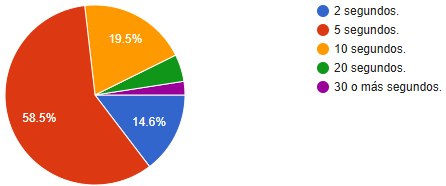
\includegraphics[width=0.7\textwidth]{images/TRF.png}
	\caption{Tiempo del proceso del reconocimiento facial.}
	\label{fig:tiempo-RF}
\end{figure}
\begin{figure}
	\centering
	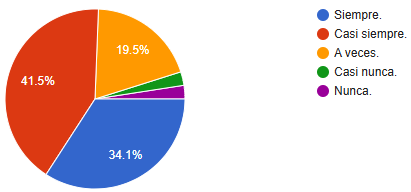
\includegraphics[width=0.7\textwidth]{images/FRF.png}
	\caption{Frecuencia de resultados correctos del reconocimiento facial.}
	\label{fig:FRF}
\end{figure}
\begin{figure}
	\centering
	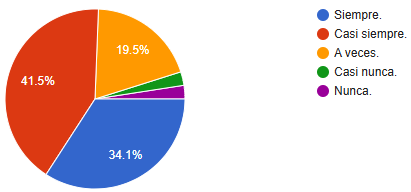
\includegraphics[width=0.7\textwidth]{images/FRF.png}
	\caption{Seguridad del alumno con la presición del reconocimiento facial.}
	\label{fig:SPRF}
\end{figure}
\begin{figure}
	\centering
	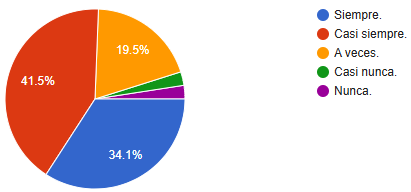
\includegraphics[width=0.7\textwidth]{images/FRF.png}
	\caption{Intentos necesarios para que el reconocimiento facial lo identificara correctamente.}
	\label{fig:IRF}
\end{figure}
\begin{figure}
	\centering
	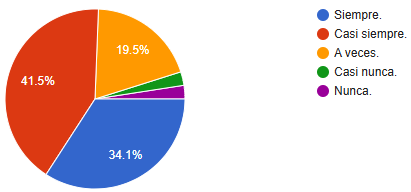
\includegraphics[width=0.7\textwidth]{images/FRF.png}
	\caption{Rapidez y fluidez del proceso del reconocimiento facial.}
	\label{fig:FRRF}
\end{figure}
\begin{figure}
	\centering
	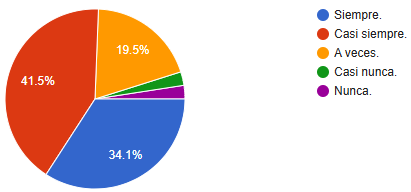
\includegraphics[width=0.7\textwidth]{images/FRF.png}
	\caption{Utilidad de la información mostrada en los detalles del ETS.}
	\label{fig:IIETS}
\end{figure}
\begin{figure}
	\centering
	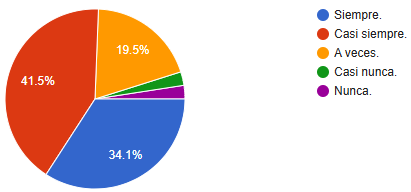
\includegraphics[width=0.7\textwidth]{images/FRF.png}
	\caption{Utilidad de las instrucciones mostradas para el ingreso de los ETS.}
	\label{fig:USIETS}
\end{figure}
\begin{figure}
	\centering
	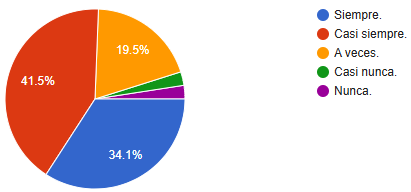
\includegraphics[width=0.7\textwidth]{images/FRF.png}
	\caption{Comodidad del usuario al navegar por la app móvil.}
	\label{fig:CNU}
\end{figure}
\begin{figure}
	\centering
	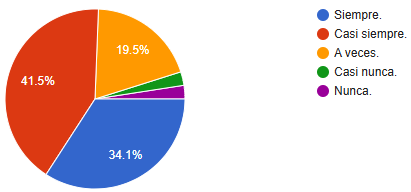
\includegraphics[width=0.7\textwidth]{images/FRF.png}
	\caption{Correcta paleta de colores.}
	\label{fig:UCA}
\end{figure}